\subsubsection{Counter weights}
\subsubsection*{Arm weight balancing}
After deciding on the section of the boom that would be fixed to the rotator, we proceeded to determine the required force and its location to neutralize the weight acting on the antenna arm for this pivot point. We found the center of gravity of the antenna and then commenced moving it backwards until it sits at the center of the upper plate where it is mounted. A mass of 0.8 kg was calculated to be required at 13.5 cm from the center (from center to center). This value varies slightly depending on the shape of the weight attached. Conveniently, we found some microphone boom weights with the same value and that also attach to the same diameter of the boom we have. However sometimes an adapter might be required, and this would have slight implications on the position of the counterweight as we take into account the additional mass in that location. Figures 400.11 and 400.12 show the counter weight options. 
\begin{figure}[H]
	\centering
	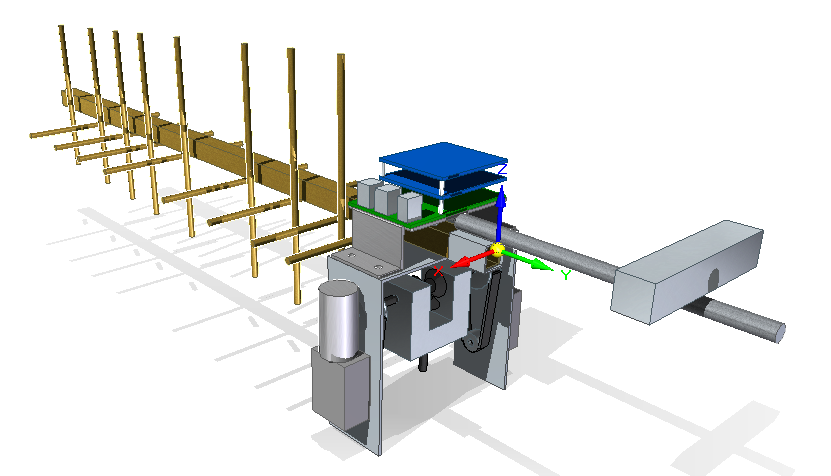
\includegraphics[width=0.5\textwidth]{../art/isoback.png}
	\caption{Arm weight balancing}
\end{figure}

\begin{figure}[H]
	\centering
	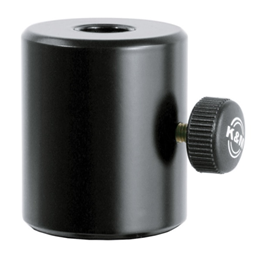
\includegraphics[width=0.2\textwidth]{../art/weight1.png}
	\caption{Commercial 0.8 kg counter weight. [2]}
\end{figure}





\subsubsection*{Pitch mass shift compensation} 
Pitch mass shift counter weights are used to balance the centre of gravity in vertical axis. The final target is to balance centre of gravity at rotational axis of the rotator. This will put negligible load on motors and motors have to overcome just inertia. The considered rotator design requires balancing of centre of gravity in both horizontal and vertical axis.  To compensate real case variations, dead weights are mounted on COTS threaded rods. This helps the user to balance the centre of gravity with extreme accuracy. Figure 400.13 shows the pitch mass weights. 


\begin{figure}[H]
	\centering
	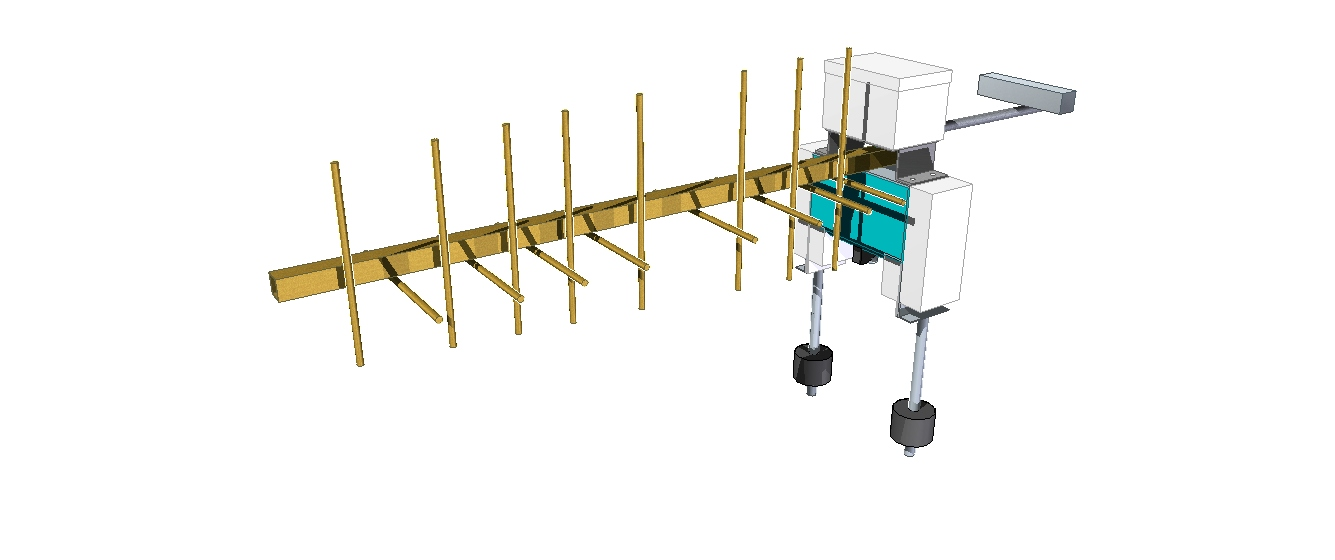
\includegraphics[width=1\textwidth]{../art/isoshield.jpg}
	\caption{Pitch mass weights}
\end{figure}
